\documentclass[]{beamer}

\title{Quasicrystals and the cut and project method}
\author{Ingmar Lowack, Noah Koopmann}
\date{\today}
\institute{Heidelberg Experimental Geometry Lab}

\begin{document}
  
\begin{frame}
  \titlepage
\end{frame}
\begin{frame}
  \tableofcontents
\end{frame}

\begin{frame}
  \section{Introduction}
  \subsection{Crystals}
  \frametitle{Crystals}
  \begin{itemize}
    \item periodic structure
    \item tiling: set of geometric shapes that fill a plane
    \item simplest crystals are constructed using regular polygons
  \end{itemize}
\end{frame}
\begin{frame}
  \frametitle{Crystals examples 1}
  \begin{figure}
    \centering
    \setlength{\fboxsep}{0pt}%
\setlength{\fboxrule}{1pt}%
        \fbox{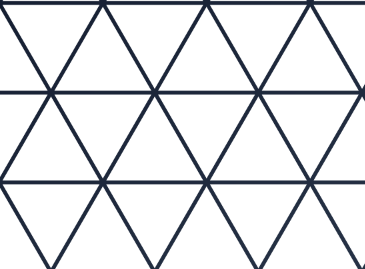
\includegraphics[width=0.3\textwidth]{assets/tilingTriangle.png}}
        \fbox{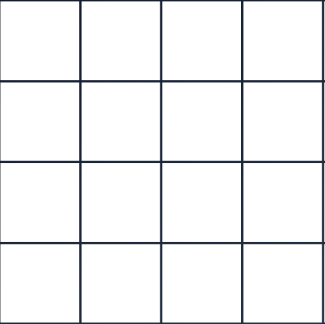
\includegraphics[width=0.3\textwidth]{assets/TilingSquare.png}}
        \fbox{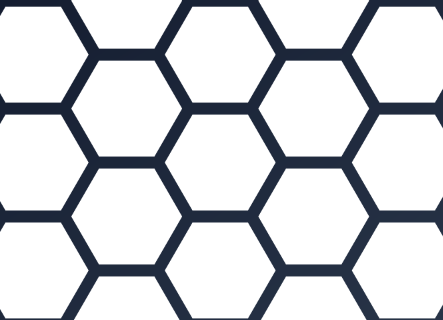
\includegraphics[width=0.3\textwidth]{assets/TilingHexagon.png}}
        \caption{from regular polygons only triangles, squares and hexagons make a crystal}
        \label{fig:periodicTilings}
    \end{figure}
\end{frame}
\begin{frame}
  \frametitle{Crystals examples 2}
  \begin{figure}
    \centering
        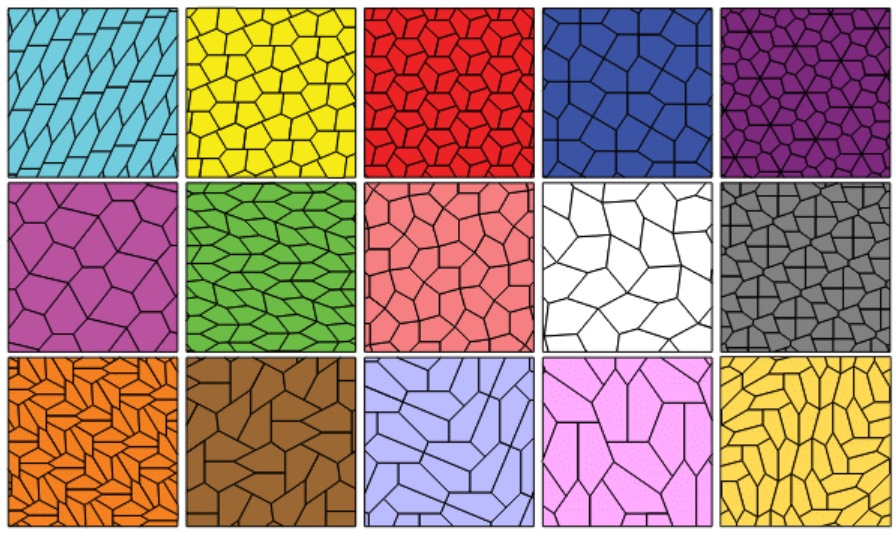
\includegraphics[width=1\textwidth]{assets/unregularTilings.png}
        \caption{periodic tilings made of unregular pentagons. Source [2] http://community.wolfram.com/groups/-/m/t/550169}
        \label{fig:periodicTilings2}
    \end{figure}
\end{frame}
\begin{frame}
  \subsection{Quasicrystals}
  \frametitle{Quasicrystals}
  \begin{itemize}
    \item quasi-periodic structure
    \item also appear in nature
    \item examples are fibonacci \& penrose tilings (coming up)
  \end{itemize}
\end{frame}
% TODO:? Quasicrystals and the golden ratio
\begin{frame}
  \section{Cut and project method}
  \subsection{General workings}
  \frametitle{Cut and project method}
  \begin{itemize}
    \item most versatile method to generate quasicrystals
    \item general working:
    \begin{enumerate}
      \item starting with an $n\geq2$ dimensional lattice $\Lambda\in \mathbb{R}^n$
      \item take a affin-linear subspace $E$ of dimension $m<n$ and \textbf{cut} $\mathbb{R}^n$
      \item \textbf{project} all points of $\Lambda$ onto $E^\perp$ and check if they fall into a certain cut window
      \item take the accepted points and project them onto $E$
    \end{enumerate}
    ...see example in next slide
  \end{itemize}
\end{frame}
\begin{frame}
  \subsection{Example 1: Fibonacci Tiling}
  \frametitle{Example 1: Fibonacci Tiling}
  \begin{columns} 
    % Column 1
        \begin{column}{.5\textwidth}
          \begin{itemize}
            \item start with 2D grid (periodic tiling)
            \item $E$ is a slope with angle $\Theta$
            \item all points in the cutwindow are projected orthogonal down
            \item we get a 1D Quasicrystal if $\Theta$ is irrational:
            \item If we choose $\Theta=\tan^{-1}(\frac{1}{\tau})$ we obtain the Fibonacci tiling ($\tau$ is the \textit{golden ratio})
          \end{itemize}
        \end{column}
    % Column 2    
        \begin{column}{.5\textwidth}
          \begin{figure}
            \centering
              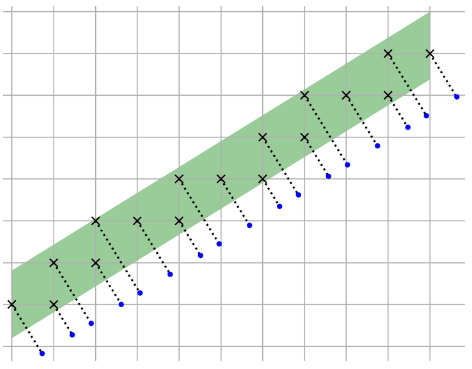
\includegraphics[width=\textwidth]{assets/fibonacci1D.png}
              \caption{fibonacci cut\&project with $\Theta=\tan^{-1}(\frac{1}{\tau})$ and $\Delta=\sin(\Theta)+\cos(\Theta)$}
              \label{fig:fibonacci1D}
            \end{figure}
        \end{column}%
        
    \end{columns}
\end{frame}
\begin{frame}
  \subsection{Example 2: Penrose Tiling}
  \frametitle{Example 2: Penrose Tiling}
  \begin{itemize}
    \item most famous Quasicrystal
    \item produced by choosing $\Lambda = \mathbb{Z}^5$ and $E$ as a certain 2 dimensional subspace of $\mathbb{R}^5$
  \end{itemize}
  \begin{figure}
    \begin{minipage}{.5\textwidth}
      \centering
      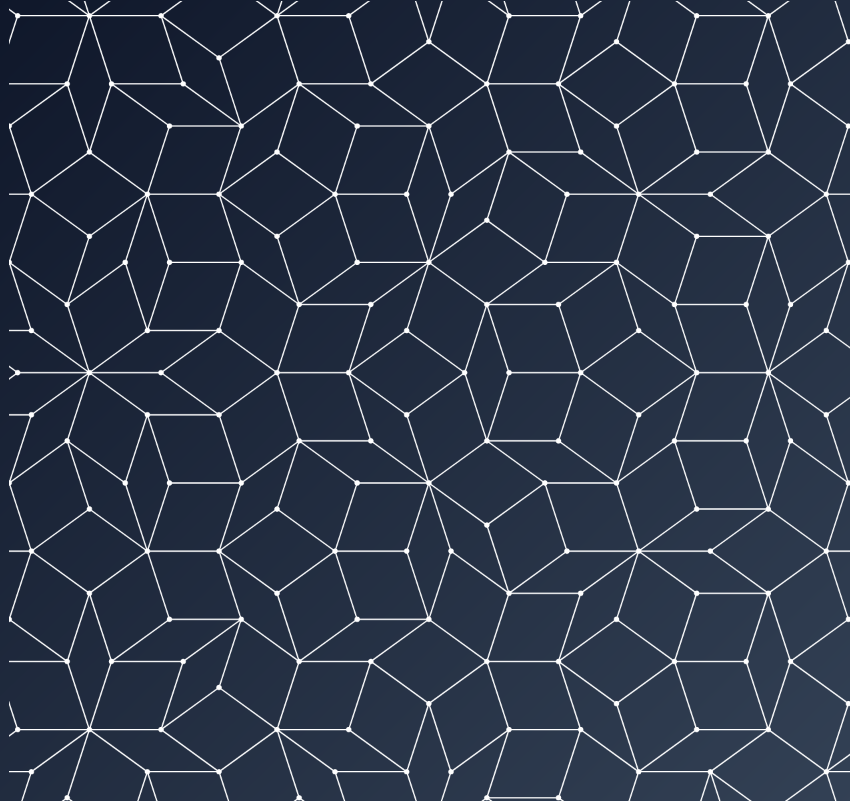
\includegraphics[width=.4\linewidth]{assets/PenroseTiling.png}
      \captionof{figure}{A figure}
      \label{fig:Penrose Tiling}
    \end{minipage}%
    \begin{minipage}{.5\textwidth}
      \centering
      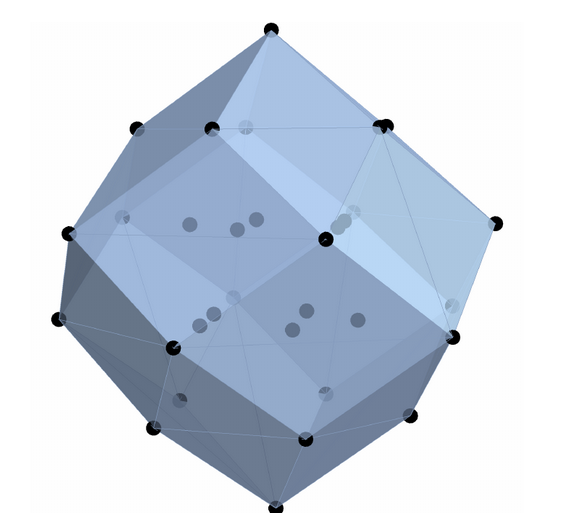
\includegraphics[width=.4\linewidth]{assets/CutWindowPenrose.png}
      \captionof{figure}{Another figure}
      \label{fig:Cut window for Penrose tiling}
    \end{minipage}
    \end{figure}
\end{frame}
\begin{frame}
  \section{Our work progress}
  \frametitle{Our work progress}
  \begin{itemize}
    \item Done:
    \begin{itemize}
      \item implemented Fibonacci tiling and Penrose tiling
      \item website with interactive tools and informative text
    \end{itemize}
    \item Next steps:
    \begin{itemize}
      \item add more interactive tools
      \item optimize penrose generation using digital geometry techniques
      \item implement further tilings such as Wang tilings
    \end{itemize}
  \end{itemize}
\end{frame}
\begin{frame}
  \section{Sources}
  \frametitle{Sources}
  Content and Figures from
  \begin{itemize}
    \item \href{http://pcwww.liv.ac.uk/~hemraj/thesis/BSc/2021_Daniel_Gouldsbrough_BSc_Thesis.pdf}{[1] 2021\_Daniel\_Gouldsbrough\_BSc\_Thesis.pdf}
    \item \href{http://community.wolfram.com/groups/-/m/t/550169}{[2] http://community.wolfram.com/groups/-/m/t/550169}
  \end{itemize}
\end{frame}

% \section{Next steps}
% \subsection{Optimize our code (penrose tiling) using digital geometry techniques}
% \subsection{Implement further tilings such as Wang tilings}

% use own images (from website)
% for the website: remove regular polygon that don't tile. Radio buttons instead of slider

\section{Showcase}
\end{document}